\clearpage
\section{Properties Of The Tangent Function}
The tangent function, like sine and cosine, has a period. But it's much easier to determine. Take a loog at the tangent function.
\begin{center}
    \begin{minipage}[c]{0.42\linewidth}
        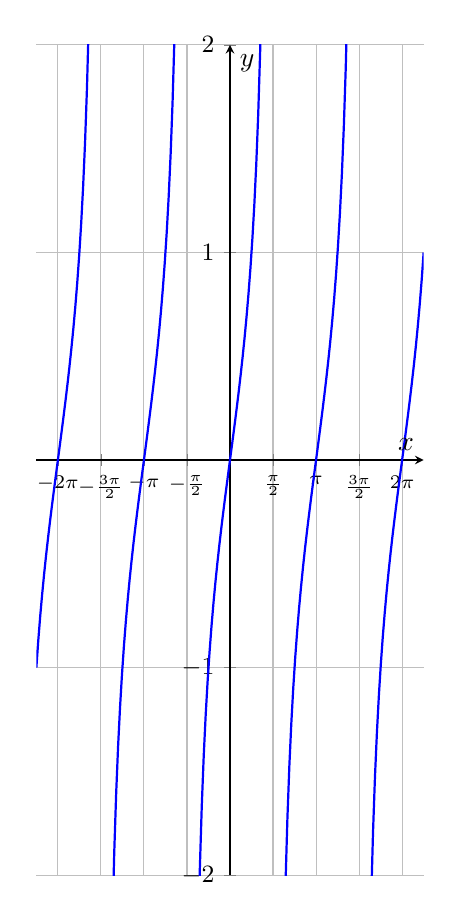
\begin{tikzpicture}
            \begin{axis}[%
                xlabel = {$x$}, ylabel = {$y$},
                xmin = {-1 * 9/4*pi}, xmax = {9/4*pi},
                ymin = -2, ymax = 2,
                restrict y to domain=-10:10,
                xtick = {
                    -2 * pi,
                    -3 / 2 * pi,
                    -1 * pi,
                    -1 / 2 * pi,
                    0, 
                    pi / 2, 
                    pi, 
                    (3 * pi) / 2,
                    2 * pi%
                    },
                xticklabels = {
                    $-2\pi$,
                    $-\frac{3\pi}{2}$,
                    $-\pi$,
                    $-\frac{\pi}{2}$,
                    $0$,
                    $\frac{\pi}{2}$,
                    $\pi$,
                    $\frac{3\pi}{2}$,
                    $2\pi$%
                },
                ytick = {
                    -2,
                    -1,
                    1,
                    2%
                },
                x tick label style = {font=\scriptsize},
                y tick label style = {font=\small},
                axis lines = center, grid = both,
                width = 6.5cm, height = \linewidth,
                trig format plots=rad
            ]
            \addplot[color = blue, thick, domain = {-1 * 9/4*pi}:{9/4*pi}, samples = 200]{tan(x)};
            \end{axis}
        \end{tikzpicture}
    \end{minipage}
    \begin{minipage}[c]{0.57\textwidth}
        Notice how it follows a consistent pattern. Each segment starts at $-\infty$, crosses the $x$-axis line at some $x = n\pi$, and then shoots up to $\infty$. And then the pattern repeats.
        \\ \\
        This pattern is why it's so easy to find the period of this function. It's just the distance between asymptotes.
    \end{minipage}
\end{center}
\begin{center}
    \begin{minipage}[c]{0.57\linewidth}
        Look at this snippet of the tangent function from $x = \frac{\pi}{2}$ to $x = \frac{3\pi}{2}$. The asymptote on the left is at $x = \frac{\pi}{2}$. The asymptote on the right is $\frac{3\pi}{2}$. So, to find the period of this, we just subtract the right asymptote by the left.
        \[
            \frac{3\pi}{2} - \frac{\pi}{2} = \pi
        \]
    \end{minipage}
    \begin{minipage}[c]{0.42\textwidth}
        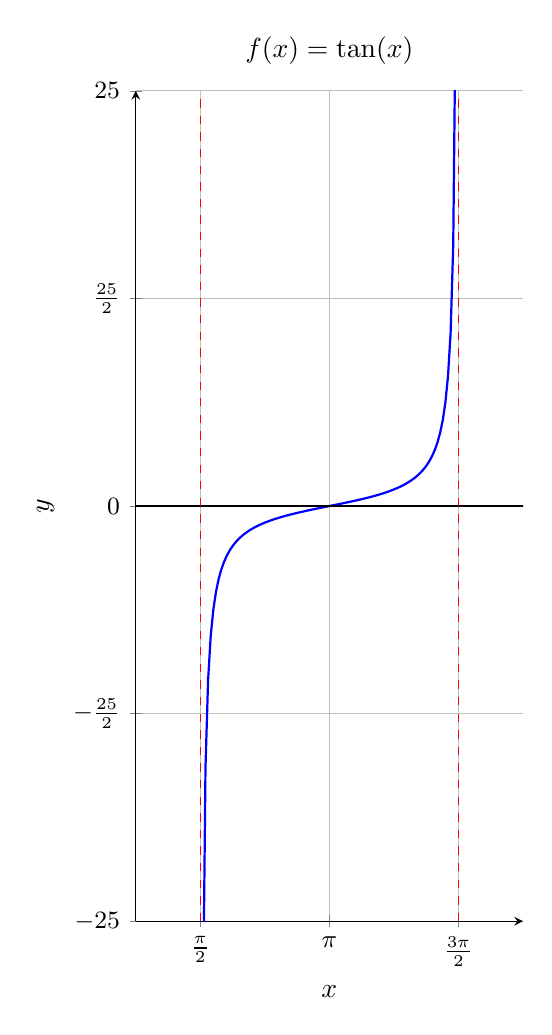
\begin{tikzpicture}
            \begin{axis}[%
                title = {$f(x) = \tan(x)$},
                xlabel = {$x$}, ylabel = {$y$},
                xmin = {pi / 4}, xmax = {(7 / 4) * pi},
                ymin = -25, ymax = 25,
                restrict y to domain=-50:50,
                xtick = {
                    -2 * pi,
                    -3 / 2 * pi,
                    -1 * pi,
                    -1 / 2 * pi,
                    0, 
                    pi / 2, 
                    pi, 
                    (3 * pi) / 2,
                    2 * pi%
                    },
                xticklabels = {
                    $-2\pi$,
                    $-\frac{3\pi}{2}$,
                    $-\pi$,
                    $-\frac{\pi}{2}$,
                    $0$,
                    $\frac{\pi}{2}$,
                    $\pi$,
                    $\frac{3\pi}{2}$,
                    $2\pi$%
                },
                ytick = {
                    -25,
                    -12.5,
                    0,
                    12.5,
                    25%
                },
                yticklabels = {
                    $-25$,
                    $-\frac{25}{2}$,
                    $0$,
                    $\frac{25}{2}$,
                    $25$%
                },
                x tick label style = {font=\small},
                y tick label style = {font=\small},
                axis lines = left, grid = both,
                width = 6.5cm, height = \linewidth,
                trig format plots=rad
            ]
            \addplot[color = blue, thick, domain = {pi / 2}:{(3/2) * pi}, samples = 100]{tan(x)};
            \draw[color = black] (0, 0) -- ({2 * pi}, 0);
            \draw[color = red, dashed] ({pi / 2}, {-25}) -- ({pi / 2}, 25);
            \draw[color = red, dashed] ({(3 / 2) * pi}, {-25}) -- ({(3 / 2) * pi}, 25);
            \end{axis}
        \end{tikzpicture}
    \end{minipage}
\end{center}
That makes the period of the function $f(x) = \tan(x)$ equal to $\pi$. That's about it. To find the period of the tangent function, you just see how far appart the asymptotes are from each other.
\clearpage
Let's try a different example.
\begin{problem}
    From the graph below, determine the period of this tangent function.
    \begin{center}
        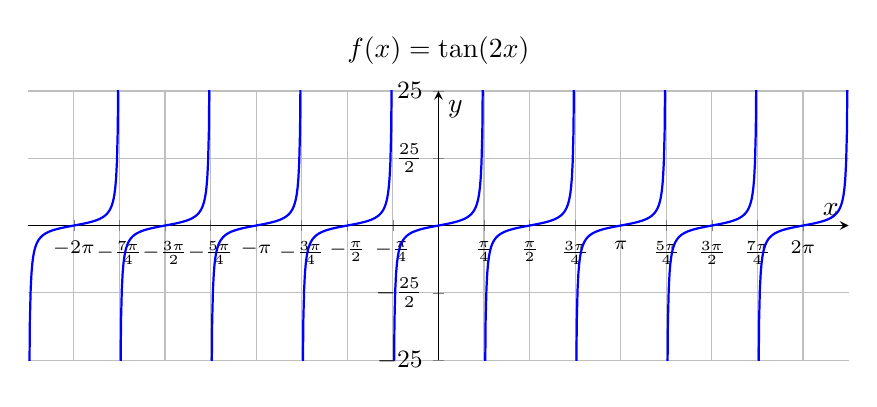
\begin{tikzpicture}
            \begin{axis}[%
                title = {$f(x) = \tan(2x)$},
                xlabel = {$x$}, ylabel = {$y$},
                xmin = {-1 * (9/4) * pi}, xmax = {9/4*pi},
                ymin = -25, ymax = 25,
                restrict y to domain=-100:100,
                xtick = {
                    -1 * 2 * pi,
                    -1 * (7 / 4) * pi,
                    -1 * (3 / 2) * pi,
                    -1 * (5 / 4) * pi,
                    -1 * pi,
                    -1 * (3 / 4) * pi,
                    -1 * (1 / 2) * pi,
                    -1 * (1 / 4) * pi,
                    0,
                    (1 / 4) * pi,
                    (1 / 2) * pi,
                    (3 / 4) * pi,
                    pi,
                    (5 / 4) * pi,
                    (3 / 2) * pi,
                    (7 / 4) * pi,
                    2 * pi%
                    },
                xticklabels = {
                    $-2\pi$,
                    $-\frac{7\pi}{4}$,
                    $-\frac{3\pi}{2}$,
                    $-\frac{5\pi}{4}$,
                    $-\pi$,
                    $-\frac{3\pi}{4}$,
                    $-\frac{\pi}{2}$,
                    $-\frac{\pi}{4}$,
                    $0$,
                    $\frac{\pi}{4}$,
                    $\frac{\pi}{2}$,
                    $\frac{3\pi}{4}$,
                    $\pi$,
                    $\frac{5\pi}{4}$,
                    $\frac{3\pi}{2}$,
                    $\frac{7\pi}{4}$,
                    $2\pi$%
                },
                ytick = {
                    -25,
                    -12.5,
                    12.5,
                    25%
                },
                yticklabels = {
                    $-25$,
                    $-\frac{25}{2}$,
                    $\frac{25}{2}$,
                    $25$%
                },
                x tick label style = {font=\scriptsize},
                y tick label style = {font=\small},
                axis lines = center, grid = both,
                width = 12cm, height = 5 cm,
                trig format plots=rad
            ]
            \addplot[color = blue, thick, domain = {-1 * 9/4*pi}:{9/4*pi}, samples = 1000] {tan(2 * x)};
            \end{axis}
        \end{tikzpicture}
    \end{center}
\end{problem}
\begin{solution}
    \begin{center}
        \begin{minipage}[c]{0.5\linewidth}
            \begin{tikzpicture}
                \begin{axis}[%
                    xlabel = {$x$}, ylabel = {$y$},
                    xmin = pi / 4, xmax = (3 * pi) / 4,
                    ymin = -25, ymax = 25,
                    restrict y to domain=-50:50,
                    xtick = {
                        -2 * pi,
                        -3 / 2 * pi,
                        -1 * pi,
                        -1 / 2 * pi,
                        0, 
                        pi / 2, 
                        pi, 
                        (3 * pi) / 2,
                        2 * pi%
                        },
                    xticklabels = {
                        $-2\pi$,
                        $-\frac{3\pi}{2}$,
                        $-\pi$,
                        $-\frac{\pi}{2}$,
                        $0$,
                        $\frac{\pi}{2}$,
                        $\pi$,
                        $\frac{3\pi}{2}$,
                        $2\pi$%
                    },
                    ytick = {
                        -25,
                        -12.5,
                        0,
                        12.5,
                        25%
                    },
                    yticklabels = {
                        $-25$,
                        $-\frac{25}{2}$,
                        $0$,
                        $\frac{25}{2}$,
                        $25$%
                    },
                    x tick label style = {font=\small},
                    y tick label style = {font=\small},
                    axis lines = middle, grid = both,
                    width = \linewidth, height = \linewidth,
                    trig format plots=rad
                ]
                \addplot[color = blue, thick, domain = {pi / 4}:{(3 / 4) * pi}, samples = 200]{tan(2 * x)};
                \end{axis}
            \end{tikzpicture}
        \end{minipage}
        \begin{minipage}[c]{0.45\textwidth}
            Notice how it follows a consistent pattern. Each segment starts at $-\infty$, crosses the $x$-axis line at some $x = n\pi$, and then shoots up to $\infty$. And then the pattern repeats.
            \\ \\
            This pattern is why it's so easy to find the period of this function. It's just the distance between asymptotes.
        \end{minipage}
    \end{center}
    Looking at the first blue line in the positive $x$ direction, we see that the left asymptote is at $x = \frac{\pi}{4}$ and the right asymptote is at $x = \frac{3\pi}{4}$.
    \[
        \frac{3\pi}{4} - \frac{\pi}{4} = \frac{2\pi}{4} = \frac{\pi}{2}
    \]
    Thus, the period of this function is $\frac{\pi}{2}$.
\end{solution}